\documentclass[10pt]{article}
\usepackage{../pplmanual}
%%% Commonly Needed packages
\usepackage{graphicx,color,calc}
\usepackage{fancyvrb}
\usepackage{makeidx}
\usepackage{alltt}
\usepackage[linkbordercolor=(0 0 1),citebordercolor=(0 1 0)]{hyperref}
%%\usepackage{xspace} <- creates problems with other hyperlink packages like "html"

%%% Commands for uniform looks of C++, Charm++, and Projections
\newcommand{\CC}{C\hbox{++}}
\newcommand{\emCC}{C\hbox{\em++}}
\newcommand{\charmpp}{\textsc{Charm++}}
\newcommand{\charmc}{\texttt{charmc}}
\newcommand{\projections}{\textsc{Projections}}
\newcommand{\converse}{\textsc{Converse}}
\newcommand{\ampi}{\textsc{AMPI}}
\newcommand{\tempo}{\textsc{TeMPO}}
\newcommand{\irecv}{\textsl{iRecv}}
\newcommand{\sdag}{\textsl{Structured Dagger}}
\newcommand{\jade}{Jade}

%%% Commands to produce margin symbols
\newcommand{\new}{\marginpar{\fbox{\bf$\mathcal{NEW}$}}}
\newcommand{\important}{\marginpar{\fbox{\bf\Huge !}}}
\newcommand{\experimental}{\marginpar{\fbox{\bf\Huge $\beta$}}}

%%% Commands for manual elements
\newcommand{\zap}[1]{ }
\newcommand{\function}[1]{{\noindent{\textsf{#1}}\\}}
\newcommand{\cmd}[1]{{\noindent{\textsf{#1}}\\}}
\newcommand{\args}[1]{\hspace*{2em}{\texttt{#1}}\\}
\newcommand{\prototype}[1]{\vspace{0.2in}\index{#1}}
\newcommand{\param}[1]{{\texttt{#1}}}
\newcommand{\kw}[1]{{\textsf{#1}\index{#1}}}
\newcommand{\uw}[1]{{\textsl{#1}}}
\newcommand{\desc}[1]{\indent{#1}}
\newcommand{\note}[1]{(\textbf{Note:} #1)}
\newcommand{\term}[1]{{\bf #1}\index{#1}}

\makeindex


\makeindex

\title{\charmpp\\ Multiblock Framework\\ Manual}
\version{1.0}
\credits{
This version of \charmpp{} Multiblock Framework was developed
by Orion Lawlor and Milind Bhandarkar.
}

\begin{document}

\maketitle

\section{Motivation}
A large class of problems can be solved by first decomposing the
problem domain into a set of structured grids.  For simplicity,
each structured grid is often made rectangular, when it is called a {\em block}.
These blocks may face one another or various parts of the outside world,
and taken together comprise a {\em multiblock computation}.

There are two main types of multiblock computations-- implicit and explicit.
In an implicit computation a global matrix, which represents the entire
problem domain, is formed and solved.  Implicit computations require
a fast sparse matrix solver, and are typically used for steady-state
problems.  In an explicit computation, the solution proceeds locally,
computing new values based on the values of nearby points. Explict
computations often have stability criteria, and are typically used for
time-dependent problems.

The \charmpp{} multiblock framework allows you to write a parallel 
explicit multiblock program,
in C or Fortran 90, by concentrating on what happens to a single block
of the domain.  Boundary condition housekeeping and ``ghost cell'' exchange
are all handled transparently by the framework.
Using the multiblock framework also allows you to take advantage of all the
features of \charmpp, including adaptive computation and communication 
overlap, run-time load balancing,  performance
monitoring and visualization, and checkpoint/restart, with no additional
effort.


\section{Introduction/Terminology}
A {\em block} is a distorted rectangular grid that represents a 
portion of the problem domain.  A volumetric cell in the grid
is called a {\em voxel}.  Each exterior side of a block
is called a {\em face}. Each face may consist of several 
rectangular {\em patches}, which all abut the same block 
and experience the same boundary conditions.

\begin{figure}[h]
\begin{center}
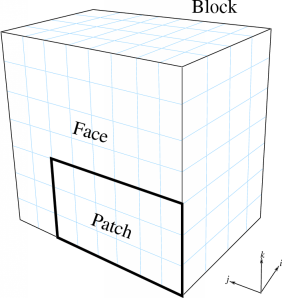
\includegraphics[width=3in]{fig/terminology}
\end{center}
\caption{Terminology used by the framework.}
\label{fig:terminology}
\end{figure}

For example, Figure~\ref{fig:terminology} shows a 3D
4x8x7-voxel block, with a face and 6x3 patch indicated.

The computational domain is tiled with such blocks, which 
are required to be conformal-- the voxels must match exactly.
The blocks need not be the same size or orientation, however,
as illustrated in the 2D domain of Figure~\ref{fig:decompose}.

\begin{figure}[h]
\begin{center}
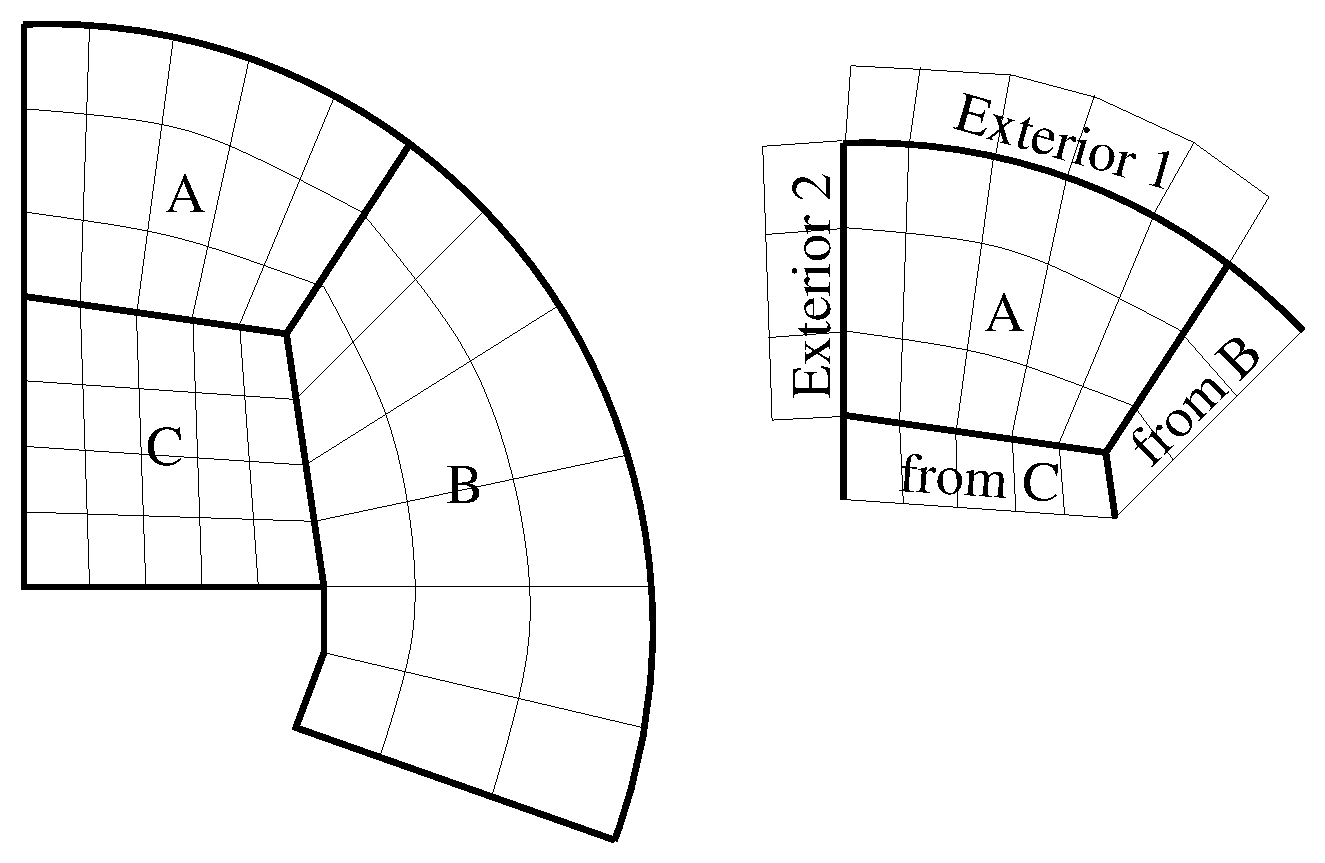
\includegraphics[width=4in]{fig/decompose}
\end{center}
\caption{A 2D domain decomposed into three blocks: A (5x3), B (3x6), 
and C (5x4). Also shows the computation as seen from block A.}
\label{fig:decompose}
\end{figure}

Figure~\ref{fig:decompose} also shows the computation 
from the point of view of block A, which has two external
boundary conditions (on the left and top sides) and two 
``internal'' boundary conditions (on the right and bottom sides).
During the computation, the external boundary conditions can
be imposed independent of any other blocks; while the internal 
boundary conditions must be obtained from the other blocks.

To simplify the computation on the interior, these boundary conditions
are typically written into special extra ``ghost'' (or dummy) cells
around the outside of the real interior cells.  The array indexing
for these ghost cells is illustrated in Figure~\ref{fig:indexing}.

\begin{figure}[h]
\begin{center}
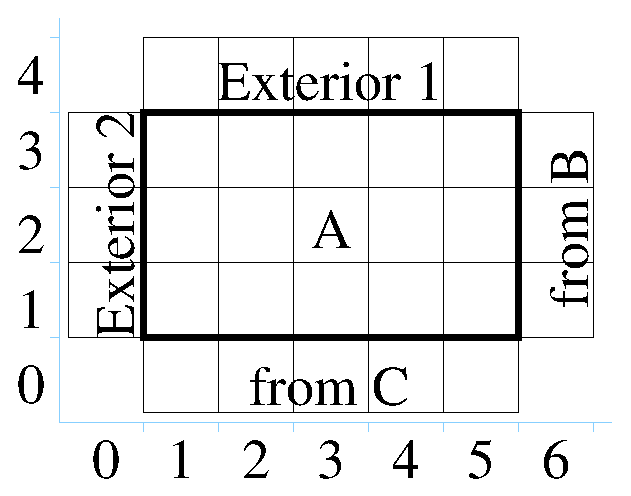
\includegraphics[width=2in]{fig/indexing}
\end{center}
\caption{The ghost cells around a 5x3-voxel 2D block}
\label{fig:indexing}
\end{figure}


The Multiblock framework manages all the boundary conditions--
both internal and external.  Internal boundary conditions are 
sent across processors, and require you to register the data 
``fields'' you wish exchanged.  External boundary conditions are
not communicated, but require you to register a function to
apply that boundary condition to your data.  Either type of boundary 
condition can have arbitrary thickness.

Finally, the Multiblock framework manages nothing {\em but} boundary conditions.
The rest of the computation, such as deciding on and implementing
timestepping, stencils, numerics, and interpolation schemes are all 
left up to the user.  

\section{Input Files}
The Multiblock framework reads, in parallel, a partitioned set of 
blocks from block input files.  Each block consists of a file
with extension ``.mblk'' for the interior data (grid coordinates
and initial conditions) and ``.bblk'' for the boundary condition data
(patches where boundaries should be applied).

These block files are generated with a separate, offline tool
called ``makemblock'', which is documented elsewhere.

\section{Structure of a Multiblock Framework Program}

A Multiblock framework program consists of several subroutines: \kw{init}, \kw{driver},\kw{finalize}, and external boundary condition subroutines.  

\kw{init} and \kw{finalize} are called by the Multiblock framework only on the first processor -- these routines typically do specialized I/O, startup and shutdown tasks.  

A separate \kw{driver} subroutine runs for each block, and does the main work of the program.  Because there may be several blocks per processor, several \kw{driver} routines may be executing as threads simultaniously.  

The boundary condition subroutines are called by the framework after a 
request from \kw{driver}.


\begin{alltt}
     subroutine init
          read configuration data
     end subroutine

     subroutine bc1
          apply first type of boundary condition
     end subroutine bc1

     subroutine bc2
          apply second type of boundary condition
     end subroutine bc2

     subroutine driver
          allocate and initialize the grid
          register boundary condition subroutines bc1 and bc2
          time loop
               apply external boundary conditions
               apply internal boundary conditions
               perform serial internal computation
          end time loop
     end subroutine

     subroutine finalize
           write results
     end subroutine
\end{alltt}



\section{Compilation and Execution}

A Multiblock framework program is a \charmpp\ program, so you must begin by
downloading the latest source version of \charmpp\ from
{\tt http://charm.cs.uiuc.edu/}.  Build the source with 
{\tt ./build MBLOCK version} or {\tt cd} into the build directory, 
{\tt version/tmp}, and type {\tt make MBLOCK}.
To compile a MULTIBLOCK program, pass the {\tt -language mblock} (for C) or 
{\tt -language mblockf} (for Fortran) option to {\tt charmc}.

In a charm installation, see charm/version/pgms/charm++/mblock/
for example and test programs.


\section{Multiblock Framework API Reference}

The Multiblock framework is accessed from a program via a set of routines.
These routines are available in both C and Fortran90 versions.
The C versions are all functions, and always return an error code of 
MBLK\_SUCCESS or MBLK\_FAILURE.
The Fortran90 versions are all subroutines, and take an extra integer
parameter ``err'' which will be set to MBLK\_SUCCESS or MBLK\_FAILURE.

\subsection{Initialization}
All these methods should be called from the \kw{init} function by the user. 
The values passed to these functions are typically read from a configuration 
file or computed from command-line parameters.

\vspace{0.2in}
\function{int MBLK\_Set\_prefix(const char *prefix);}
\function{subroutine MBLK\_Set\_prefix(prefix,err)}
  \args{character*, intent(in)::prefix}
  \args{integer, intent(out)::err}
This function is called to set the block filename prefix. 
For example, if the input block files are named ``gridX000001.mblk''
and ``gridX000002.mblk'', the prefix is the string ``gridX''.

\vspace{0.2in}
\function{int MBLK\_Set\_nblocks(const int n);}
\function{ subroutine MBLK\_Set\_nblocks(n,err)}
  \args{integer, intent(in)::n}
  \args{integer, intent(out)::err}
This call is made to set the number of partitioned blocks to be used.
Each block is read from an input file and a separate \kw{driver}
is spawned for each.  The number of blocks determines the available
parallelism; so be sure to have at least as many blocks as processors.
We recommend using several times more blocks than processors, to ease 
load balancing and allow adaptive overlap of computation and communication.

\vspace{0.2in}
\function{int MBLK\_Set\_dim(const int n);}
\function{subroutine MBLK\_Set\_dim(n, err)}
  \args{integer, intent(in)::n}
  \args{integer, intent(out)::err}
This call is made to set the number of spatial dimensions. 
Only three dimensional computations are currently supported.

\subsection{Utility}

\function{int MBLK\_Get\_nblocks(int* n);}
\function{subroutine MBLK\_Get\_nblocks(n,err)}
  \args{integer,intent(out)::n}
  \args{integer,intent(out)::err}
Get the total number of blocks in the current computation.  
Can only be called from the driver routine.

\vspace{0.2in}
\function{int MBLK\_Get\_myblock(int* m);}
\function{subroutine MBLK\_Get\_myblock(m,err)}
  \args{integer,intent(out)::m }
  \args{integer,intent(out)::err }
Get the id of the current block, an integer from 0 to the number of blocks minus one. 
Can only be called from the driver routine. 

\vspace{0.2in}
\function{int MBLK\_Get\_blocksize(int* dims);}
\function{subroutine MBLK\_Get\_blocksize(dimsm,err)}
  \args{integer,intent(out)::dims(3)}
  \args{integer,intent(out)::err }
Get the interior dimensions of the current block, in voxels. 
The size of the array dims should be 3, and will be filled with
the $i$, $j$, and $k$ dimensions of the block. 
Can only be called from the driver routine. 

\vspace{0.2in}
\function{double MBLK\_Timer(void);}
\function{function double precision :: MBLK\_Timer()}

Return the current wall clock time, in seconds.  Resolution is
     machine-dependent, but is at worst 10ms.

\vspace{0.2in}
\function{void MBLK\_Print\_block(void);}
\function{subroutine MBLK\_Print\_block()}
Print a debugging representation of the framework's information
about the current block.

\vspace{0.2in}
\function{void MBLK\_Print(const char *str);}
\function{subroutine MBLK\_Print(str)}
\args{  character*, intent(in) :: str}
     Print the given string, prepended by the block id if called from the 
     driver. Works on all machines; unlike \kw{printf} or
     \kw{print *}, which may not work on all parallel machines.


\subsection{Internal Boundary Conditions and Block Fields}

The Multiblock framework handles the exchange of boundary values 
between neighboring blocks.
The basic mechanism to do this exchange is the {\em field}-- numeric data items 
associated with each cell of a block. These items must be arranged in a regular
3D grid; but otherwise we make no assumptions about the meaning of a
field.

You create a field once, with \kw{MBLK\_Create\_Field}, then pass the resulting 
field ID to \kw{MBLK\_Update\_Field} (which does the
overlapping block communication) and/or \kw{MBLK\_Reduce\_Field} (which 
applies a reduction over block values).


\vspace{0.2in}
\function{int MBLK\_Create\_Field(int *dimensions,int isVoxel,const int base\_type,const int vec\_len,const int offset,const int dist, int *fid);}
\function{subroutine MBLK\_Create\_Field(dimensions, isVoxel,base\_type, vec\_len, offset, dist, err)}
  \args{integer, intent(in)  :: dimensions, isVoxel, base\_type, vec\_len, offset, dist}
  \args{integer, intent(out) :: fid, err}
     Creates and returns a Multiblock field ID, which can be passed to
\kw{MBLK\_Update\_Field} and \kw{MBLK\_Reduce\_Field.}  Can only be called from
\kw{driver().}  

     \kw{dimensions} describes the size of the array the field is in.
	Dimensions is itself an array of size 3, giving the $i$, $j$, and $k$ sizes.
	The size should include the ghost regions-- i.e., pass the actual allocated
	size of the array.
     \kw{isVoxel} describes whether the data item is to be associated with
	a voxel (1, a volume-centered value) or the grid corners (0, a corner-centered
	value). 
     \kw{base\_type} describes the type of each data item, one of:

     \begin{itemize}
        \item \kw{MBLK\_BYTE}-- unsigned char, INTEGER*1, or CHARACTER*1
        \item \kw{MBLK\_INT}-- int or INTEGER*4
        \item \kw{MBLK\_REAL}-- float or REAL*4
        \item \kw{MBLK\_DOUBLE}-- double, DOUBLE PRECISION, or REAL*8
     \end{itemize}

     \kw{vec\_len} describes the number of data items associated with each
     cell, an integer at least 1.

     \kw{offset} is the byte offset from the start of the array to the
     first interior cell's data items, a non-negative integer.  
     This can be calculated using the \kw{offsetof()} function; normally with
     \kw{offsetof(array(1,1,1),array(interiorX,interiorY,interiorZ))}.  
     Be sure to skip over any ghost regions.

     \kw{dist} is the byte offset from the first cell's data items to the
     second, a positive integer (normally the size of the data items).
     This can also be calculated using \kw{offsetof()}; normally with 
	\kw{offsetof(array(1,1,1),array(2,1,1))}.

     \kw{fid} is the identifier for the field that is created by the function.

\vspace{0.2in}
In the example below, we register a single double-precision value with
each voxel.  The ghost region is 2 cells deep along all sides.

\begin{alltt}
	!In Fortran
	double precision, allocatable :: voxData(:,:,:)
	integer :: size(3), ni,nj,nk
 	integer :: fid, err

	!Find the dimensions of the grid interior
	MBLK_Get_blocksize(size,err);

	!Add ghost region width to the interior dimensions 
	size=size+4;  ! 4 because of the 2-deep region on both sides 

	!Allocate and initialize the grid 
	allocate(voxData(size(1),size(2),size(3)))
	voxData=0.0

	!Create a field for voxData
	call MBLK_Create_field(&
	       &size,1, MBLK_DOUBLE,3,&
	       &offsetof(grid(1,1,1),grid(3,3,3)),&
	       &offsetof(grid(1,1,1),grid(2,1,1)),fid,err)	
	

\end{alltt}
     This example uses the Fortran-only helper routine \kw{offsetof}, which
     returns the offset in bytes of memory between its two given
     variables.  C users can use the built-in \kw{sizeof} keyword or pointer
     arithmetic to achieve the same result.

\vspace{0.2in}
\function{void MBLK\_Update\_field(const int fid,int ghostwidth, void *grid);}
\function{subroutine MBLK\_Update\_field(fid,ghostwidth, grid,err)}
  \args{integer, intent(in)  :: fid, ghostwidth}
  \args{integer,intent(out) :: err}
  \args{varies, intent(inout) :: grid}

     Update the values in the ghost regions specified when the
     field was created.  This call sends this block's interior region out,
     and receives this block's boundary region from adjoining blocks.

     Ghostwidth controls the thickness of the ghost region. To only exchange
     one cell on the boundary, pass 1.  To exchange two cells, pass 2. 
     To include diagonal regions, make the ghost width negative.
     A ghost width of zero would communicate no data.

\begin{figure}[h]
\begin{center}
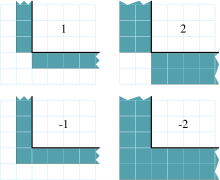
\includegraphics[width=2in]{fig/ghostwidth}
\end{center}
\caption{The 2D ghost cells communicated for various ghost widths.  The heavy line
is the block interior boundary-- this is the lower left portion of the block.}
\label{fig:ghostwidth}
\end{figure}      

     \kw{MBLK\_Update\_field} can only be called from driver, and to be useful,
     must be called from every block's driver routine.

     \kw{MBLK\_Update\_field} blocks till the field has been updated.
     After this routine returns, the given field will updated.
     If the update was successful MBLK\_SUCCESS is returned and 
     MBLK\_FAILURE is returned in case of error.

\vspace{0.2in}
\function{void MBLK\_Iupdate\_field(const int fid,int ghostwidth, void *ingrid, void* outgrid);}
\function{subroutine MBLK\_Iupdate\_field(fid,ghostwidth, ingrid, outgrid,err)}
  \args{integer, intent(in)  :: fid, ghostwidth}
  \args{integer,intent(out) :: err}
  \args{varies,intent(in) :: ingrid}
  \args{varies,intent(out) :: outgrid}
     Update the values in the ghost regions which were specified when the
     field was created. For the example above the ghost regions will be 
     updated once for each step in the time loop.

     \kw{MBLK\_Iupdate\_field} can only be called from driver, and to be useful,
     must be called from every block's driver routine.

     \kw{MBLK\_Iupdate\_field} is a non blocking call similar to MPI\_IRecv.
     After the routine returns the update may not yet be complete; and the
     outgrid may be in an inconsistent state.  Before using the values the 
     status of the
     update must be checked using \kw{MBLK\_Test\_update} or 
     \kw{MBLK\_Wait\_update}.

     There can be only one outstanding iupdate call in progress at any time.
     
\vspace{0.2in}
\function{int MBLK\_Test\_update(int *status);}
\function{subroutine MBLK\_Test\_update(status,err)}
\args{integer, intent(out) :: status,err}
     \kw{MBLK\_Test\_update} is a call that is used in association with 
     \kw{MBLK\_Iupdate\_field} from the driver sub routine.  It tests whether
      the preceeding iupdate has completed or not.
     \kw{status} is returned as MBLK\_DONE if the update was completed or 
      MBLK\_NOTDONE if the update is still pending.
     Rather than looping if the update is still pending, call \kw{MBLK\_Wait\_update}
     to relinquish the CPU.

\vspace{0.2in}
\function{void MBLK\_Wait\_update(void);}
\function{subroutine MBLK\_Wait\_update()}
     \kw{MBLK\_Wait\_update} call is a blocking call and is used in assoication 
     with \kw{MBLK\_Iupdate\_field} call. It blocks until the update is completed.

\vspace{0.2 in}
\function{void MBLK\_Reduce\_field(int fid,void *grid, void *out,int op);}
\function{subroutine MBLK\_Reduce\_field(fid,grid,outVal,op)}
  \args{integer, intent(in)  :: fid,op}
  \args{varies, intent(in) :: grid}
  \args{varies, intent(out) :: outVal}
     Combine a field from each block, according to op, across all blocks.
     Only the interior values of the field will be combined; not the ghost cells.
     After \kw{Reduce\_Field} returns, all blocks will have identical
values in \kw{outVal,} which must be \kw{vec\_len} copies of \kw{base\_type}.


     May only be called from driver, and to complete, must be called
     from every chunk's driver routine.

     \kw{op} must be one of:

\begin{itemize}
        \item \kw{MBLK\_SUM}-- each element of \kw{outVal} will be the sum 
of the corresponding fields of all blocks
        \item \kw{MBLK\_MIN}-- each element of \kw{outVal} will be the 
smallest value among the corresponding field of all blocks
        \item \kw{MBLK\_MAX}-- each element of \kw{outVal} will be the largest 
value among the corresponding field of all blocks
\end{itemize}

\vspace{0.2in}
\function{void MBLK\_Reduce(int fid,void *inVal,void *outVal,int op);}
\function{subroutine MBLK\_Reduce(fid,inVal,outVal,op)}
  \args{integer, intent(in)  :: fid,op}
  \args{varies, intent(in) :: inVal}
  \args{varies, intent(out) :: outVal}
     Combine a field from each block, acoording to \kw{op}, across all blocks.
\kw{Fid} is only used for the \kw{base\_type} and \kw{vec\_len}-- offset and
\kw{dist} are not used.  After this call returns, all blocks will have
identical values in \kw{outVal}.  Op has the same values and meaning as
\kw{MBLK\_Reduce\_Field}.
     May only be called from driver, and to complete, must be called
     from every blocks driver routine.

\vspace{0.2in}

\subsection{External Boundary Conditions}

Most problems include some sort of boundary conditions.  These conditions
are normally applied in the ghost cells surrounding the actual computational domain.
Examples of boundary conditions are imposed values, reflection walls, symmetry planes,
inlets, and exits.

The Multiblock framework keeps track of where boundary conditions are to be applied.
You register a subroutine that the framework will call to apply each type of 
external boundary condition.

\vspace{0.2in}
\function{int MBLK\_Register\_bc(const int bcnum, int ghostWidth, const MBLK\_BcFn bcfn);}
\function{subroutine MBLK\_Register\_bc(bcnum, ghostwidth, bcfn, err)}
\args{integer,intent(in) :: bcnum, ghostWidth}
\args{integer,intent(out) :: err}
\args{subroutine :: bcfn}
This is call is used to bind an external boundary condition subroutine,
written by you, to a boundary condition number.
\kw{MBLK\_Register\_bc} should only be called from the driver.

\begin{itemize}
	\item \kw{bcnum} The boundry condtion number to be associated with the 
	function.
	\item \kw{ghostWidth} The width of the ghost cells where this boundry
	condition is to be applied.
	\item \kw{bcfn} The user subroutine to be called to apply this
	boundry condition.
\end{itemize}

When you ask the framework to apply boundary conditions, it will call this
routine.  The routine should be declared like:

\begin{alltt}
	!In Fortran
	subroutine applyMyBC(param1,param2,start,end)
	varies :: param1, param2
	integer :: start(3), end(3)
	end subroutine

	/* In C */
	void applyMyBC(void *param1,void *param2,int *start,int *end);	
\end{alltt}
 
\kw{param1} and \kw{param2} are not used by the framework-- they are
passed in unmodified from \kw{MBLK\_Apply\_bc} and \kw{MBLK\_Apply\_bc\_all}.
\kw{param1} and \kw{param2} typically contain the block data and dimensions.  

\kw{start} and \kw{end} are 3-element arrays that give the $i$,$j$, $k$ 
block locations where the boundary condition
is to be applied.  They are both inclusive and both relative to the 
block interior-- you must shift them over your ghost cells.  The C versions
are 0-based (the first index is zero); the Fortran versions are 1-based
(the first index is one).  

For example, a Fortran subroutine to apply the constant value 1.0 across the
boundary, with a 2-deep ghost region, would be:

\begin{alltt}
	!In Fortran
	subroutine applyMyBC(grid,size,start,end)
	integer :: size(3), i,j,k
	double precision :: grid(size(1),size(2),size(3))
	integer :: start(3), end(3)
	start=start+2 ! Back up over ghost region
	end=end+2
	do i=start(1),end(1)
	do j=start(2),end(2)
	do k=start(3),end(3)
	    grid(i,j,k)=1.0
	end do
	end do
	end do

	end subroutine	
\end{alltt}


\vspace{0.2in}
\function{ int MBLK\_Apply\_bc(const int bcnum, void *param1,void *param2);}
\function{subroutine MBLK\_Apply\_bc(bcnum, param1,param2,err)}
  \args{integer,intent(in)::bcnum}
  \args{varies,intent(inout)::param1}
  \args{varies,intent(inout)::param2}
  \args{integer,intent(out)::err}
\kw{MBLK\_Apply\_bc} call is made to apply all boundry condition functions
of type \kw{bcnum} to the block.  \kw{param1} and \kw{param2} are passed unmodified
to the boundary condition function.

\vspace{0.2in}
\function{ int MBLK\_Apply\_bc\_all(void* param1, void* param2);} 
\function{subroutine MBLK\_Apply\_bc\_all(param1,param2, err)}
  \args{integer,intent(out)::err}
  \args{varies,intent(inout)::param1}
  \args{varies,intent(inout)::param2}
This call is same as \kw{MBLK\_Apply\_bc} except it applies all 
external boundary conditions to the block.


\subsection{Migration}

The \charmpp\ runtime framework includes an automated, run-time load balancer,
which will automatically monitor the performance of your parallel program.
If needed, the load balancer can ``migrate'' mesh chunks from heavily-loaded
processors to more lightly-loaded processors, improving the load balance and
speeding up the program.  For this to be useful, pass the \kw{+vpN} argument
with a larger number of blocks \kw{N} than processors
Because this is somewhat involved, you may refrain from calling 
\kw{MBLK\_Migrate} and migration will never take place.

The runtime system can automatically move your thread stack to the new
processor, but you must write a PUP function to move any global or
heap-allocated data to the new processor (global data is declared at file scope
or \kw{static} in C and \kw{COMMON} in Fortran77; heap allocated data comes
from C \kw{malloc}, C++ \kw{new}, or Fortran90 \kw{ALLOCATE}).  A PUP
(Pack/UnPack) function performs both packing (converting heap data into a
message) and unpacking (converting a message back into heap data).  All your
global and heap data must be collected into a single block (\kw{struct} in C;
user-defined \kw{TYPE} in Fortran) so the PUP function can access it all.

Your PUP function will be passed a pointer to your heap data block and a
special handle called a ``pupper'', which contains the network message to be
sent.  Your PUP function returns a pointer to your heap data block.  In a PUP
function, you pass all your heap data to routines named \kw{pup\_type}, where
type is either a basic type (such as int, char, float, or double) or an array
type (as before, but with a ``s'' suffix).  Depending on the direction of
packing, the pupper will either read from or write to the values you pass--
normally, you shouldn't even know which.  The only time you need to know the
direction is when you are leaving a processor or just arriving.
Correspondingly, the pupper passed to you may be deleting (indicating that you
are leaving the processor, and should delete your heap storage after packing),
unpacking (indicating you've just arrived on a processor, and should allocate
your heap storage before unpacking), or neither (indicating the system is
merely sizing a buffer, or checkpointing your values).

PUP functions are much easier to write than explain-- a simple C heap block
and the corresponding PUP function is:

\begin{alltt}
     typedef struct {
       int n1;/*Length of first array below*/
       int n2;/*Length of second array below*/
       double *arr1; /*Some doubles, allocated on the heap*/
       int *arr2; /*Some ints, allocated on the heap*/
     } my_block;
 
     my_block *pup_my_block(pup_er p,my_block *m)
     {
       if (pup_isUnpacking(p)) m=malloc(sizeof(my_block));
       pup_int(p,\&m->n1);
       pup_int(p,\&m->n2);
       if (pup_isUnpacking(p)) {
         m->arr1=malloc(m->n1*sizeof(double));
         m->arr2=malloc(m->n2*sizeof(int));
       }
       pup_doubles(p,m->arr1,m->n1);
       pup_ints(p,m->arr2,m->n2);
       if (pup_isDeleting(p)) {
         free(m->arr1);
         free(m->arr2);
         free(m);
       }
       return m;
     }
\end{alltt}

This single PUP function can be used to copy the \kw{my\_block} data into a
message buffer and free the old heap storage (deleting pupper); allocate
storage on the new processor and copy the message data back (unpacking pupper);
or save the heap data for debugging or checkpointing.

A Fortran block TYPE and corresponding PUP routine is as follows:

\begin{alltt}
     MODULE my_block_mod
       TYPE my_block
         INTEGER :: n1,n2x,n2y
         REAL*8, POINTER, DIMENSION(:) :: arr1
         INTEGER, POINTER, DIMENSION(:,:) :: arr2
       END TYPE
     END MODULE
 
     SUBROUTINE pup_my_block(p,m)
       IMPLICIT NONE
       USE my_block_mod
       USE pupmod
       INTEGER :: p
       TYPE(my_block) :: m
       call pup_int(p,m%n1)
       call pup_int(p,m%n2x)
       call pup_int(p,m%n2y)
       IF (pup_isUnpacking(p)) THEN
         ALLOCATE(m%arr1(m%n1))
         ALLOCATE(m%arr2(m%n2x,m%n2y))
       END IF
       call pup_doubles(p,m%arr1,m%n1)
       call pup_ints(p,m%arr2,m%n2x*m%n2y)
       IF (pup_isDeleting(p)) THEN
         DEALLOCATE(m%arr1)
         DEALLOCATE(m%arr2)
       END IF
     END SUBROUTINE
\end{alltt}

\function{int MBLK\_Register(void *block, MBLK\_PupFn pup\_ud, int* rid)}
\function{subroutine MBLK\_Register(block,pup\_ud, rid)}
    \args{integer, intent(out)::rid}
    \args{TYPE(varies), POINTER :: block}
    \args{SUBROUTINE :: pup\_ud}
     Associates the given data block and PUP function.  Returns a block
     ID, which can be passed to \kw{MBLK\_Get\_registered} later.  Can only be
     called from driver.  It returns MBLK\_SUCESS if the call was successful
     and MBLK\_FAILURE in case of error. For the declarations above, you call
     \kw{MBLK\_Register} as:

\begin{alltt}
          /*C/C++ driver() function*/
	  int myId, err;
          my_block *m=malloc(sizeof(my_block));
          err =MBLK_Register(m,(MBLK_PupFn)pup_my_block,&rid);
 
          !- Fortran driver subroutine
          use my_block_mod
          interface
            subroutine pup_my_block(p,m)
              use my_block_mod
              INTEGER :: p
              TYPE(my_block) :: m
            end subroutine
          end interface
          TYPE(my_block) :: m
          INTEGER :: myId,err
          MBLK_Register(m,pup_my_block,myId,err)
\end{alltt}

     Note that Fortran blocks must be allocated on the stack in driver;
     while C/C++ blocks may be allocated on the heap.
\vspace{0.2in}

\function{void MBLK\_Migrate()}
\function{subroutine MBLK\_Migrate()}
     Informs the load balancing system that you are ready to be
     migrated, if needed.  If the system decides to migrate you, the
     PUP function passed to \kw{MBLK\_Register} will be called with a sizing
     pupper, then a packing, deleting pupper.  Your stack (and pupped
     data) will then be sent to the destination machine, where your PUP
     function will be called with an unpacking pupper.  \kw{MBLK\_Migrate}
     will then return, whereupon you should call \kw{MBLK\_Get\_registered} to
     get your unpacked data block.  Can only be called from driver.



\function{int MBLK\_Get\_Userdata(int n, void** block)}
     Return your unpacked userdata after migration-- that is, the
     return value of the unpacking call to your PUP function.  Takes
     the userdata ID returned by \kw{MBLK\_Register}.  Can be called from
     driver at any time.

     Since Fortran blocks are always allocated on the stack, the system
     migrates them to the same location on the new processor, so no
     \kw{Get\_registered} call is needed from Fortran.
\input{index}
\end{document}
